\documentclass{beamer}
%\documentclass[handout]{beamer}
\usepackage[hungarian]{babel}
\uselanguage{hungarian}
\languagepath{hungarian}
\deftranslation[to=hungarian]{Theorem}{T\'etel}
\deftranslation[to=hungarian]{Example}{P\'elda}
\deftranslation[to=hungarian]{Definition}{Defin\'ici\'o}
%\usepackage[magyar]{babel}
\usepackage[utf8]{inputenc}

\usepackage[T1]{fontenc}
\usepackage{beamerthemesplit}
\usepackage{pgf,pgffor,pgfplots}
\pgfplotsset{compat=1.16}
\usepackage{subfig}
\usepackage{xcolor}

\usepackage{listings}
\usepackage{nccfoots}
\newcommand{\framenote}[1]{%
	\Footnotetext{}{\emph{#1}}% Print footnote text
}

\makeatletter
\let\old@lstKV@SwitchCases\lstKV@SwitchCases
\def\lstKV@SwitchCases#1#2#3{}
\makeatother
\usepackage{lstlinebgrd}
\AtBeginEnvironment{figure}{\setcounter{subfigure}{0}}
\makeatletter
%%%%%%%%%%%%%%%%%%%%%%%%%%%%%%%%%%%%%%%%%%%%%%%%%%%%%%%%%%%%%%%%%%%%%%%%%%%%%%
%
% \btIfInRange{number}{range list}{TRUE}{FALSE}
%
% Test in int number <number> is element of a (comma separated) list of ranges
% (such as: {1,3-5,7,10-12,14}) and processes <TRUE> or <FALSE> respectively

\newcount\bt@rangea
\newcount\bt@rangeb

\newcommand\btIfInRange[2]{%
	\global\let\bt@inrange\@secondoftwo%
	\edef\bt@rangelist{#2}%
	\foreach \range in \bt@rangelist {%
		\afterassignment\bt@getrangeb%
		\bt@rangea=0\range\relax%
		\pgfmathtruncatemacro\result{ ( #1 >= \bt@rangea) && (#1 <= \bt@rangeb) 
		}%
		\ifnum\result=1\relax%
		\breakforeach%
		\global\let\bt@inrange\@firstoftwo%
		\fi%
	}%
	\bt@inrange%
}
\newcommand\bt@getrangeb{%
	\@ifnextchar\relax%
	{\bt@rangeb=\bt@rangea}%
	{\@getrangeb}%
}
\def\@getrangeb-#1\relax{%
	\ifx\relax#1\relax%
	\bt@rangeb=100000%   \maxdimen is too large for pgfmath
	\else%
	\bt@rangeb=#1\relax%
	\fi%
}

%%%%%%%%%%%%%%%%%%%%%%%%%%%%%%%%%%%%%%%%%%%%%%%%%%%%%%%%%%%%%%%%%%%%%%%%%%%%%%
%
% \btLstHL<overlay spec>{range list}
%
% TODO BUG: \btLstHL commands can not yet be accumulated if more than one 
%overlay spec match.
% 
\newcommand<>{\btLstHL}[1]{%
	\only#2{\btIfInRange{\value{lstnumber}}{#1}{\color{orange!30}\def\lst@linebgrdcmd{\color@block}}{\def\lst@linebgrdcmd####1####2####3{}}}%
}%
\makeatother

\usepackage{hyperref}
\hypersetup{
    colorlinks = true,
    linkcolor = blue,
    urlcolor  = blue,
    citecolor = blue,
    linkbordercolor = {white},
}
\usepackage{alltt}
\usepackage{tikz}
\usetikzlibrary{arrows,automata}
\usetheme{Warsaw}
\institute{Szegedi Tudományegyetem}
\pgfdeclareimage[height=0.55cm]{institution-logo}{../szte_logo}
\logo{\pgfuseimage{institution-logo}}

\title{Algoritmusok és adatszerkezetek II.}
\subtitle{Sztring,-és számelméleti algoritmusok}
\date{}

\begin{document}

\maketitle

\begin{frame}{Mintaillesztés problémája}
$T=[t_1 \ldots t_n]$ input tartalmazza-e a $P=[p_1 \ldots p_m]$ 
mintát? Ha igen, mely inputpozíció(k)tól/eltolási érték(ek)től 
kezdődően?\\
Tipikusan $n \gg m$

\only<2>{
\begin{example}
	Hányszor szerepel az \texttt{'orosz'} szó a \textit{Háború és béke} c. 
	műben?
\end{example}

Nyers erőt használva legrosszabb esetben $O(mn)$ vizsgálat kell
Milyen hatékonyabb módszerek vannak?
\begin{itemize}
	\item Mintaillesztés automatával
	\item Knuth-Morris-Prat	
	\item \textbf{Rabin-Karp algoritmus}
\end{itemize}
}
\end{frame}

\begin{frame}{Jelölések}
\begin{itemize}
	\item $\mathtt{P}_i$ jelölje \texttt{P}-nek az $i$ hosszúságú prefixét 
	(kezdőszeletét), azaz pl. $\mathtt{P}_3=bab$, $\mathtt{P}_1=b$, illetve 
	$\mathtt{P}_0=\epsilon$ ($\epsilon$ az üres szót jelöli)
	\item<2-> $\mathtt{X} \sqsupset \mathtt{Y}$ jelölje azt, ha \texttt{X} 
	sztring szuffixe \texttt{Y}-nak (azaz \texttt{Y} végződése maga \texttt{X})
	\begin{block}<2->{Példa}
		$\mathtt{\underline{aaba}}\sqsupset\mathtt{cac\underline{aaba}}$, 
		ugyanakkor 
		$\mathtt{\underline{aaba}}\not\sqsupset\mathtt{cac\underline{aab\textcolor{red}{\textbf{b}}}}$\\
		Megjegyzés: Az $\mathtt{Y} \sqsupset \mathtt{Y}$, valamint az $\epsilon 
		\sqsupset \mathtt{Y}$ relációk triviálisan teljesülnek minden 
		$\mathtt{Y}$-ra.
	\end{block}
\end{itemize}
\end{frame}

\begin{frame}{Véges állapotú automaták}
	Automata alatt egy $M=(Q,q_0,A,\Sigma,\delta)$ rendezett ötöst értünk, ahol
\begin{itemize}
	\item $Q$ a lehetséges állapotok halmaza
	\item $q_0$ a kezdőállapot
	\item $A\subseteq Q$ a végállapotok halmaza
	\item $\Sigma$ egy véges ábécé
	\item $\delta: Q \times \Sigma \rightarrow Q$ az 
	állapotátmenet-függvény
\end{itemize}
\end{frame}

\begin{frame}{Mintaillesztés véges állapotú automatákkal}
 \begin{itemize}
 	\item $Q$-t válasszuk $\{q_0, q_1, \ldots q_m \}$-nak
 	\item $q_i$ állapot jelentése: az input aktuális pozíciójáig a minta első 
 	$i$ karaktere illeszkedik
	\item $q_m$ állapotba elérve elmondható, hogy megtaláltuk a $P$-nek egy 
	$T$-beli előfordulását
 \end{itemize}
\end{frame}

\begin{frame}[fragile]{$\delta$ kiszámítása}
\begin{alltt}
{\scshape{ÁtmenetFüggvénySzámítás}}(P, \(\Sigma\)) \{
  m = P.length
  for (q = 0 to m) \{
    for (\(a\in\Sigma\)) \{
      k = min(m + 1, q + 2)
      repeat
        k = k - 1
      until \(\mathtt{P\textsubscript{k}}\sqsupset\mathtt{P\textsubscript{q}}a\)
      \(\delta(q, a) = k\)
    \}
  \}
  return \(\delta\)
\}
\end{alltt}
\end{frame}

\begin{frame}{$P=baba$ minta felismerését végző véges automata}

\begin{block}{Az állapotátmenet-függvény táblázatos formában}
\begin{table}
	\centering
\begin{tabular}{c|ccccc}
	& $q_0$ & $q_1$ & $q_2$ & $q_3$ & $q_4$ \\ \hline
	a & $q_0$ & $\mathbf{q_2}$ & $q_0$ & $\mathbf{q_4}$ & $q_0$ \\
	b & $\mathbf{q_1}$ & $q_1$ & $\mathbf{q_3}$ & $q_1$ & $q_3$ \\
\end{tabular}
\end{table}
Kitöltése és tárolása egyaránt $O(m \lvert \Sigma \rvert)$ költségű
\end{block}

\begin{figure}
	\begin{tikzpicture}[>=stealth',auto,node distance=2cm]
	\node[initial,state]         (q0) {$q_0$};
	\node[state]         (q1) [right of=q0] {$q_1$};
	\node[state]         (q2) [right of=q1] {$q_2$};
	\node[state]         (q3) [right of=q2] {$q_3$};
	\node[state,accepting] (q4) [right of=q3] {$q_4$};
	
	\path[->]
	(q0) edge node {b} (q1)
	edge [loop below,color=red] node {a} (q0)
	(q1) edge [color=red]node {a} (q2)
	edge[loop above] node {b} (q1)
	(q2) edge node {b} (q3)
	edge [bend left, color=red] node {a} (q0)
	(q3) edge [color=red] node {a} (q4)
	edge [bend right=60]  node {b} (q1)
	(q4) edge [bend left=60,color=red] node {a} (q0)
	edge [bend left] node {b} (q3);
	\end{tikzpicture}
\end{figure}
\end{frame}

\begin{frame}{Knuth-Morris-Pratt (KMP) algoritmus}
\begin{block}{A véges automatával történő feldolgozás korlátai}
	Előfeldolgozás gyanánt ki kell tölteni egy $m\lvert \Sigma \rvert$ méretű 
	táblázatot (és persze tárolni is kell azt)
\end{block}
\begin{block}<2>{Észrevételek}
	\begin{enumerate}
		\item Ha $P=aab$ minta illeszkedett az input $i$-edik pozíciójára, 
		akkor az $i+1$ pozíciótól kezdődően biztos nem beszélhetünk 
		illeszkedésről
		\item Ha $P=aaa$ minta nem illeszkedett az input $i$-edik
		pozíciójára, akkor az $i+1$ pozíciótól kezdődően biztos nem 
		beszélhetünk illeszkedésről
	\end{enumerate}
\end{block}
\end{frame}

\begin{frame}{Prefixfüggvény}
\begin{itemize}
	\item $\pi: \{1,2,\ldots,m\} \rightarrow \{0,1,\ldots,m-1\}$ $P=[p_1\ldots 
	p_m]$ minta prefixfüggvénye, ha $\pi[q]=\max\{k : k 
	< q \wedge \mathtt{P}_k \sqsupset \mathtt{P}_q\}$
	\item Azaz $\pi[q]$ megadja \texttt{P} azon leghosszabb ($q$-nál rövidebb) 
	prefixének hosszát, ami valódi szuffixe	$\mathtt{P}_q=[p_0\ldots p_q]$-nak
	\item Értelmezése: ha \textbf{nem sikerül továbbillesszük} a mintát az 
	inputra, az \textbf{legalább} mely állapotig vet minket vissza
\end{itemize}
\begin{block}<2>{Példa}
	$T=abaabababaca$ inputban keressük a $P=a b a b a b a b c a$ mintát
	\begin{table}
		\centering
		\begin{tabular}{c|cccccccccc}
		$i$ & 1 & 2 & 3 & 4 & 5 & 6 & 7 & 8 & 9 & 10 \\ \hline
	$P[i]$  & a & b & a & b & a & b & a & b & c & a \\
	$\pi[i]$& 0 & 0 & 1 & 2 & 3 & 4 & 5 & 6 & 0 & 1
		
		\end{tabular}
	\end{table}
\end{block}
\end{frame}

\begin{frame}{A prefixfüggvény növekedése}
\begin{alertblock}{}
	Indirekt belátható, hogy $\pi[i+1] - \pi[i] \leq 1$ minden esetben teljesül

\pause
\centering
$\underbrace{\overbrace{s_1 ~ s_2}^{\pi[i] = 2} ~ s_3 ~ s_4}_{\pi[i+1] = 4} ~ 
\dots ~ \underbrace{s_{i-2} ~ \overbrace{s_{i-1} ~ s_{i}}^{\pi[i] = 2} ~ 
s_{i+1}}_{\pi[i+1] = 4}$
\end{alertblock}

\begin{block}{}
	Azaz $\pi[i+1] - \pi[i] > 1$ csak úgy teljesülhet, ha $\pi[i]$ nem 
	$\mathtt{P}_i$ leghosszabb valódi szuffixének a hossza, ami ellentmondás.
\end{block}
\end{frame}

\begin{frame}{Prefixfüggvény viselkedése}
\begin{itemize}
	\item Folytatódó illeszkedés \\
		$\underbrace{\overbrace{s_1 ~ s_2 ~ s_3}^{\pi[i]} ~ 
		\overbrace{\color{red}{s_4}}^{s_4 = s_{i+1}}}_{\pi[i+1] = \pi[i] + 1} ~ 
		\dots ~ 
		\underbrace{\overbrace{s_{i-2} ~ s_{i-1} ~ s_{i}}^{\pi[i]} ~ 
		\overbrace{\color{red}{s_{i+1}}}^{s_4 = s_i + 1}}_{\pi[i+1] = \pi[i] + 
		1}$
	\item Nem (közvetlen) folytatódó illeszkedés
	$\overbrace{\underbrace{s_1 ~ s_2}_j ~ s_3 ~ s_4}^{\pi[i]} ~ \dots ~ 
	\overbrace{s_{i-3} ~ s_{i-2} ~ \underbrace{s_{i-1} ~ 
	s_{i}}_{j=\pi[\pi[i]]}}^{\pi[i]} ~ 
	s_{i+1}$
\end{itemize}
\end{frame}

\begin{frame}[fragile]{Prefixfüggvény kiszámítása}
\begin{alltt}
{\scshape{PrefixSzámít}}(P) \{
  m = P.length
  \(\pi[1]=0\)
  i = 0
  for (q=2 to m) \{
    while i > 0 and P[i+1] \(\neq\) P[q]
      i = \(\pi\)[i]
    if P[i+1] = P[q]
      i = i+1
    \(\pi\)[q]=i
  \}
  return \(\pi\)
\} 
\end{alltt}
\end{frame}

\begin{frame}[fragile]{KMP algoritmus}
\begin{alltt}
{\scshape{KMP-illesztő}}(T, P) \{
  n = T.length
  m = P.length
  \(\pi\) = {\scshape{PrefixSzámít}}(P)
  q = 0 
  for (i = 1 to n)
    while q > 0 and P[q + 1] \(\neq\) T [i]
      q = \(\pi\)[q]
    if P[q + 1] = T [i]
      q = q + 1
    if q = m
      print("Illeszkedés a \%d. pozícióval bezárólag" \% i)
      q = \(\pi\)[m]
\}
\end{alltt}
\end{frame}

\begin{frame}{Rabin-Karp algoritmus}
Az egyszerűség kedvéért a mintára és az inputra tekintsünk 10-es 
számrendszerbeli számokként
\begin{block}{Alapötlet}
	$P$ mintára alkalmazzunk egy $h_q(x) = x \mod q$ hasítófüggvényt.
	$T$-nek csak azon $S=[t_j]_{j=i}^{i+m-1}$ réssztringjei egyezhetnek meg 
	$P$-vel, melyekre $h_q(S)=h_q(P)$\\
	$h_q(S)=h_q(P)$ természetesen csak szükségességi feltételt támaszt
\end{block}
\end{frame}

\begin{frame}{Rabin-Karp algoritmus illusztráció (Forrás: CLRS 32.5 ábra)}
$P=31415, h_q(x) = x \mod 13$
\begin{figure}
\centering
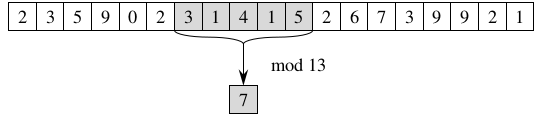
\includegraphics[width=.8\linewidth]{RK1}
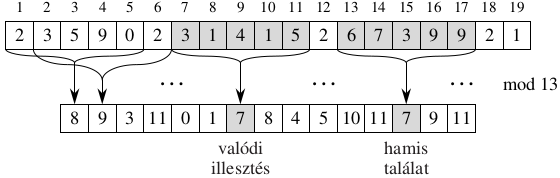
\includegraphics[width=.8\linewidth]{RK2}
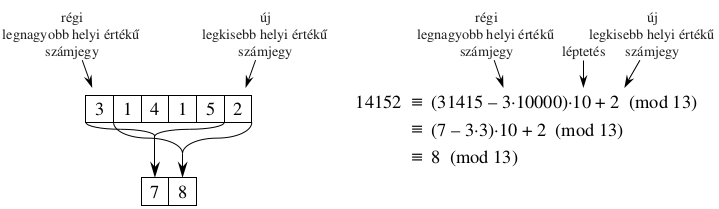
\includegraphics[width=.8\linewidth]{RK3}
\end{figure}
\end{frame}

\begin{frame}{Rabin-Karp -- a hasítófüggvény csúsztatása}
\begin{alertblock}{Észrevétel}
	$h_q$-nak az input minden indexén kezdődő kiszámítása költséges
\end{alertblock}
\begin{block}<2>{A hatékonyság záloga}
	Ahogy $abc$ és $bcd$ számpárral teljesül $$bcd 
	= 10*(abc - 100*a) + d$$ egyenlőség, hasonlóan igaz $$h_q(bcd) = 
	h_q(10*(h_q(abc) 
	- h_q(100) * a) + d)$$ összefüggés is.
\end{block}
\end{frame}

\begin{frame}{Kis kitérő: Bloom filterek}
\begin{itemize}
	\item Probabilisztikus adatszerkezet a {\scshape{Keres}} műveletre 
	nézve
	\item Implementációja: (egyenletesen szóró) $h$ hasítófüggvény és 
	egy (kezdetben csupa 0) bitvektor
	\begin{itemize}
		\item $x$ elem beszúrásakor a bitvektor $h(x)$ indexét 1-re állítjuk
		\item $x$ elem keresésnél ha a bitvektor $h(x)$ indexe 1, 
		akkor azt mondjuk, hogy $x$-et tartalmazza a bloom filterünk
		\begin{itemize}
			\item Hamis elutasítás soha nem teszünk, ugyanakkor hamis pozitív 
		választ adhatunk
		\end{itemize}
	\end{itemize}
	\item Hatékonysága függ $h$ hasítófüggvénytől, valamint az eltárolt elemek 
	számától (ami kihat a bitvektor kitöltöttségére)
	\item Linkek: \href{http://billmill.org/bloomfilter-tutorial/}{Bloom filter 
	demo} és \href{http://code.google.com/p/guava-libraries/}{Guava API}
\end{itemize}
\end{frame}

\begin{frame}{Bloom filterek tévesztési arányának elemzése}
\begin{itemize}
	\item Egy bloom filter olyan arányban ad egy elem tartalmazására nézve 
	igenlő választ, mint amennyi bitje egyesre lett állítva a beszúrások 
	hatására
	\begin{itemize}
		\item Feltesszük, hogy az alkalmazott $h$ hasítófüggvény jól szór, 
		azaz $m$ ekvivalenciaosztályba való sorolás esetén az objektumok
		közelítőleg $\frac{1}{m}$ részét sorolja az összes osztályba
	\end{itemize}
	\begin{block}{Hány bitje lesz egy $m$ hosszú bloom filternek 1-es $n$ 
	beszúrás után?}
1 beszúrás során $\frac{1}{m}$ valószínűséggel töltünk föl egy bitet \\
1 beszúrás során $1-\frac{1}{m}$ valószínűséggel \textit{nem} töltünk föl egy 
bitet \\
$n$ beszúrás során $\Big(1-\frac{1}{m}\Big)^n$ valószínűséggel \textit{nem} 
töltünk föl egy bitet \\ \pause
$\Big(1-\frac{1}{m}\Big)^n=\Big[\Big(1-\frac{1}{m}\Big)^m\Big]^\frac{n}{m} 
\approx e^{-\frac{n}{m}}$ (nagy $m$ esetén)\\
$n$ beszúrást követően $1-e^{-\frac{n}{m}}$ valószínűséggel lesz a bloom filter 
valamely bitje 1-esre állítva \\ 
	\end{block}
\end{itemize}
\end{frame}

\begin{frame}{Mintaillesztés főbb megközelítései}
\begin{table}
	\centering
	\begin{tabular}{l|cc}
		Algoritmus  & Előfeldolgozás & Illesztés\footnote{legrosszabb eset} \\ 
		\hline \hline
		Nyers erő   &        0       & $O(mn)$ \\
		Rabin-Karp  &  $\Theta(m)$   & $O(mn)$ \\ \hline
		Véges automata    &  $O(m\lvert \Sigma \rvert)$   & $\Theta(n)$ \\
		Knuth-Morris-Prat &  $\Theta(m)$   & $\Theta(n)$ \\		
	\end{tabular}
\end{table}

\begin{itemize}
	\item Rabin-Karp a nyers erő módszerének heurisztikus kiterjesztéseként 
	tekinthető
	\item KMP pedig a véges automatákkal való illesztés egy hatékonyabb verziója
\end{itemize}	
\end{frame}

\begin{frame}{A moduláris hatványozás}

\begin{block}{Alapprobléma: Mi az $a^b \mod n$ kifejezés értéke?}
	Gyakorlati jelentőség: titkosító eljárások (pl.~RSA) használata során 
	szükségünk lehet ilyen számítások elvégzésére \\
\end{block}

\begin{alertblock}{}
	Már viszonylag kis $b$-re is rengeteg bitműveletet kell elvégezzünk
\end{alertblock}

\pause
\begin{block}<2>{Példa -- Mi lesz $7^{560} \mod 561$ értéke? Avagy }
179846672920572906577258722224560336083856608137007342561
612636144396089769552955665549135995604075608096691162101
184113545972526638255004784055311390598542305958357097082
391225061077433281620117130013826448606281708665937931659
796736755253074977366471063146923373865223501532185753076
292710887401801774392779475679510556311966981952826025487
057204699261913973664257857993744045143447531121540574215
969802961003872086163860991702035506591312847029674260362
509156745965136001 mod 561=?
\end{block}
\end{frame}

\begin{frame}[fragile]{Moduláris hatványozás}
\begin{columns}
	\begin{column}{.6\linewidth}
\begin{alltt}
{\scshape{Moduláris-hatványozó}}(a, b, n)\{
  \colorbox{blue!20!black!30!red}{c = 0}
  d = 1
  \colorbox{blue!20!black!30!green}{B = [bk \ldots b1 b0]}
  for (i=k; k >=0; --k) \{
    \colorbox{blue!20!black!30!red}{c = 2*c}
    d = (d*d) mod n
    if (B[i] == 1) \{
      \colorbox{blue!20!black!30!red}{c = c+1}
      d = (d*a) mod n
    \}
  \}
  return d
\}
\end{alltt}
	\end{column}
\begin{column}{.51\linewidth}
	\begin{block}{Megjegyzések}
		\begin{enumerate}
			\item $b$-nek $k$ bites bináris alakja $B$
			\item $c$ csak egy segédváltozó
		\end{enumerate}
	\end{block}

	\begin{alertblock}<2->{Kérdés}
	\begin{itemize}
		\item Mi lesz $d$ és $c$ értéke a for ciklus első végrehajtása után?
	\end{itemize}
\end{alertblock}
\begin{block}<3>{Műveletigény}
	Ha $a,b$ és $n$ $k$ biten elfér, mindez $O(k)$ aritmetikai 
	műveletet és $O(k^3)$ bitműveletet jelent
\end{block}
\end{column}
\end{columns}
\end{frame}

\begin{frame}{A moduláris hatványozás működése}
\begin{itemize}
	\item Az algoritmus for ciklusában minden egyes iteráció megkezdése előtt a 
	$c$ és $d$ változók értékeire teljesül, hogy:
	\begin{enumerate}
		\item $c$ változó értéke megegyezik a $[b_{k} \ldots b_{i+1}]$ bináris 
		értékkel
		\item $d = a^c \mod n$
	\end{enumerate}
    \item A fenti ciklusinvariáns teljesül, megmarad és befejeződik 
    $\rightarrow$ 
\end{itemize}
\end{frame}

\begin{frame}{Moduláris hatványozás példa}
\begin{block}{$7^{560} mod 561 =?$}
	$a=7, b=560, n=561$ ($B=[1000110000]$)
	\begin{table}
		\centering
		\begin{tabular}{c|cccccccccc}
         $i$ & 9 & 8 & 7 & 6 & 5 & 4 & 3 & 2 & 1 & 0 \\ \hline
       $b_i$ & 1 & 0 & 0 & 0 & 1 & 1 & 0 & 0 & 0 & 0 \\ \hline
         $c$ & 1 & 2 & 4 & 8 & 17 & 35 & 70 & 140 & 280 & 560 \\ \hline
         $d$ & 7 & 49 & 157 & 526 & 160 & 241 & 298 & 166 & 67 & 
         \boxed{\textbf{1}}
		\end{tabular}
	\end{table}
\end{block}
\end{frame}
\end{document}